% --------------------------------------------------------------
%     DENNE MALEN ER LAGET AV MARTIN SORIA RØVANG
%     TIL BRUK FOR OPPGAVELØSNINGER OG RAPPPRTER
%     GITHUB: github.com/martinrovang
% --------------------------------------------------------------


\documentclass[10pt]{article}
\usepackage{amsmath,amsthm,amssymb}
\usepackage{float}
\usepackage[norsk]{babel}
\usepackage[table]{xcolor}
\usepackage{color}
\usepackage{graphicx}
\usepackage{listings}
\usepackage{natbib}
\usepackage[utf8]{inputenc}
\usepackage{imakeidx}
\usepackage[a4paper]{geometry}
\usepackage[myheadings]{fullpage}
\usepackage{fancyhdr}
\usepackage{lastpage}
\usepackage{graphicx, wrapfig, subcaption, setspace, booktabs}
\usepackage[T1]{fontenc}
\usepackage[font=small, labelfont=bf]{caption}
\usepackage{fourier}
\usepackage[protrusion=true, expansion=true]{microtype}
\usepackage{url, lipsum}
\usepackage{tgbonum}
\usepackage{hyperref}
\usepackage{xcolor}
\usepackage[most]{tcolorbox}
\usepackage{mathtools}
\usepackage[page]{totalcount}
\usepackage{lastpage}


\newcommand{\HRule}[1]{\rule{\linewidth}{#1}}
\onehalfspacing
\setcounter{tocdepth}{5}
\setcounter{secnumdepth}{5}
\newcommand{\vect}[1]{\boldsymbol{#1}}

\definecolor{codegreen}{rgb}{0,0.6,0}
\definecolor{codegray}{rgb}{0.5,0.5,0.5}
\definecolor{codepurple}{rgb}{0.58,0,0.82}
\definecolor{backcolour}{rgb}{0.95,0.95,0.92}
\definecolor{skyblue}{rgb}{0.950, 1, 1}

\lstdefinestyle{mystyle}{
    backgroundcolor=\color{backcolour},   
    commentstyle=\color{codegreen},
    keywordstyle=\color{magenta},
    numberstyle=\tiny\color{codegray},
    stringstyle=\color{codepurple},
    basicstyle=\footnotesize,
    breakatwhitespace=false,         
    breaklines=true,                 
    captionpos=b,                    
    keepspaces=true,                 
    numbers=left,                    
    numbersep=5pt,                  
    showspaces=false,                
    showstringspaces=false,
    showtabs=false,                  
    tabsize=2,
    frame=single,
    %keywordstyle=\color{blue},
    language=Python,
    backgroundcolor = \color{skyblue}
}
 
\lstset{style=mystyle}
\lstset{
    basicstyle=\footnotesize\ttfamily,
  identifierstyle=\bfseries\color{green!40!black},
  commentstyle=\itshape\color{purple!40!black},
  keywordstyle=\color{blue},
  stringstyle=\color{orange},
}

\newcommand{\N}{\mathbb{N}}
\newcommand{\Z}{\mathbb{Z}}
 
\newenvironment{theorem}[2][Theorem]{\begin{trivlist}
\item[\hskip \labelsep {\bfseries #1}\hskip \labelsep {\bfseries #2.}]}{\end{trivlist}}
\newenvironment{lemma}[2][Lemma]{\begin{trivlist}
\item[\hskip \labelsep {\bfseries #1}\hskip \labelsep {\bfseries #2.}]}{\end{trivlist}}
\newenvironment{exercise}[2][Exercise]{\begin{trivlist}
\item[\hskip \labelsep {\bfseries #1}\hskip \labelsep {\bfseries #2.}]}{\end{trivlist}}
\newenvironment{problem}[2][Problem]{\begin{trivlist}
\item[\hskip \labelsep {\bfseries #1}\hskip \labelsep {\bfseries #2.}]}{\end{trivlist}}
\newenvironment{question}[2][Question]{\begin{trivlist}
\item[\hskip \labelsep {\bfseries #1}\hskip \labelsep {\bfseries #2.}]}{\end{trivlist}}
\newenvironment{corollary}[2][Corollary]{\begin{trivlist}
\item[\hskip \labelsep {\bfseries #1}\hskip \labelsep {\bfseries #2.}]}{\end{trivlist}}

\newenvironment{solution}{\begin{proof}[Solution]}{\end{proof}}
    
\makeindex[columns=3, title=Alphabetical Index, intoc]


% --------------------------------------------------------------
%                         Headers and footers
% --------------------------------------------------------------
\fancyhf{}
\pagestyle{fancy}
\rhead{Martin Soria Røvang}
\lhead{STA-2003-Tidsrekker}
\rfoot{Side \thepage \, av \pageref{LastPage}}
\renewcommand{\headrulewidth}{0.3pt}

\usepackage{amssymb}
\usepackage{gensymb}
\usepackage{amsmath}

% $\medblackstar \medwhitestar$

\begin{document}
% --------------------------------------------------------------
%                         FRONTPAGE
% --------------------------------------------------------------
{\fontfamily{cmr}\selectfont
\title{ \normalsize \textsc{}
		\\ [1.0cm] % How much upper margin
		%\HRule{0.5pt} \\
        \LARGE \textbf{\uppercase{Home Exam}
        \HRule{0.5pt} \\ [0.5cm]
        FYS-2010-Digital image processing
        %\HRule{2pt} \\ [0.5cm]
        \\
		\normalsize \today \vspace*{5\baselineskip}}
		}

        \date{}
\author{
		Candidate number: 25 \\ 
        University of Tromsø \\}

% \begin{titlepage}
\clearpage\maketitle
\vspace{0.2\textheight}
{\centering
Contains \pageref{LastPage} \, pages, including frontpage.\par
}
\thispagestyle{empty}
% \end{titlepage}

\newpage
\tableofcontents


% --------------------------------------------------------------
%                         TODOS
% F�rste oppgave
% --------------------------------------------------------------


% --------------------------------------------------------------
%                         Start here
% --------------------------------------------------------------

% Replace this text with your summary/reflection of ``The Secret to Raising Smart Kids".  Your total reflection should be roughly a page long.
% \cite{alpaydin_2014}

\newpage

\section{Part A}
\subsection{1}

We have the operators, $S_{1} = [-1,0,1]$ and $S_{2} = [1,2,1]$.

forming the outer product of the vectors we get,
\begin{equation*}
    g_{x} = s_{1}\otimes s_{2} =     \begin{bmatrix}
        -1\cdot1       & -1\cdot2 & -1\cdot1 \\
         0\cdot1 & 0\cdot2 & 0\cdot1 \\
        1\cdot1 & 1\cdot2 & 1\cdot1
    \end{bmatrix}
\end{equation*}

which yields,
\begin{equation}
    g_{x}  = \begin{bmatrix}
        -1       & -2 & -1 \\
         0 & 0 & 0 \\
        1 & 2 & 1
    \end{bmatrix}
\end{equation}

and $g_{y} = s_{1}\otimes s_{2}$ yields,

\begin{equation}
    g_{y}  = \begin{bmatrix}
        -1       & 0 & 1 \\
         -2 & 0 & 2 \\
        -1 & 0 & 1
    \end{bmatrix}
\end{equation}

These are the Sobel operators.
\subsection{2}

In (b) the operator $g_{x}$ is used as it increases the edges in the y-direction, the reason for this is that we have zeros in the center and in horizontal direction. When we convolve we then get the changes in the y-direction assigned to the pixel (top and bottom difference in the matrix). In image (c) the $g_{y}$ kernel has been used as it has enhanced the x-directional edges.


\subsection{3}
The bit plane which represents the most significant bits are the one with most details which is $b_{7}$. By setting the two least significant bits to zero shift the intensities to only be $4\cdot k$ intensity, where k is an integer. So here we would only have 4 shades between the intensities in the image. (the human eye cannot perceive the difference of abrupt change of such few intensities [p.626 \cite{dip}]). The histogram would look like figure(\ref{hist})
\begin{figure}[!htb]
    {\centering
        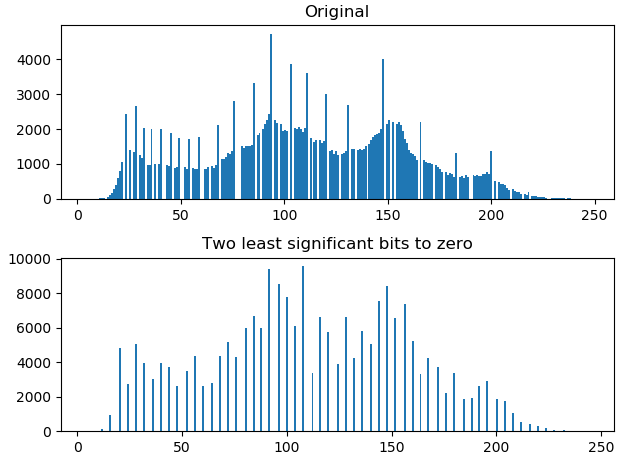
\includegraphics[width=0.70\textwidth]{bits.png}
        \caption{How the histogram changes when setting the two least significant bits(LSB) to zero. Observe how the intensities are shifted to its closest intensity which does not use the last two bits $(1,2,3) \rightarrow [01,10,11]$ every intensity from 3 to 1 is also zero.}
        \label{hist}
    \par}
    \end{figure}


    \subsection{4}

    Each pixel in an 8-bit image consist a byte consisting of numbers between 1 and 0, example $[1,1,1,0,0,0,0,0]$, we have bit planes $b_{0}-b_{7}$, where $b_{7}$ is the most significant bit plane. If we have a pixel with the byte, $[1,0,0,0,0,0,0]$ its intensity in integer values is 128. If we only allow the last bit to change and rest always zero, $[1,\underbrace{0,0,0,0,0,0}_{always = 0}]$ then we either have the intensity 0 or 128. All values above 128-255 will use the last bit in combination with the other bits, therefore we do the following transformation,
    
    \begin{equation}
        T(r) =  \begin{cases} 
            0 \, r\in\{0\leq r \leq 127 \} \\
            1 \, r\in\{128\leq r \leq 255 \}
         \end{cases}
    \end{equation}
    
    This will be the most significant bit-plane as it contains the most intensities. Its also possible to store information of the two most significant bits of an watermark and place them into the least significant bits of the original image, and the two last bits are insignificant in how a person perceive the image, you can watermark images without anyone seeing it. This can then be retrieved with an algorithm.
    
    
    \subsection{5}
    
    To invert the image we want the follow conditions: black -> white and white -> black.
    As intensity values representations: 0 -> 255 and 255 -> 0
    
    Using the transformation equation given,
    
    \begin{equation*}
        T(r) = ar + b
    \end{equation*}
    
    Putting in the conditions,
    
    \begin{equation}
        T(255) = a\cdot 255 + b = 0
        \label{transformed1}
    \end{equation}
    \begin{equation*}
        T(0) = a\cdot 0 + b = 255 => b = 255
    \end{equation*}
    
    Putting b back into equation(\ref{transformed1}) we get,
    
    \begin{equation*}
        T(255) = a\cdot 255 + 255 = 0
    \end{equation*}
    
    which yields the solution
    
    \begin{equation}
        T(r) = -r + 255
    \end{equation}





\section{Part B}
\subsection{1}
Spatial aliasing is loss of information by not using sufficient sampling rate, depending on the change of frequencies in the intensities one want to have an image of. This follows from the Nyquist sampling which says we need to sample with $f_{s} = 2f$ where f is the \emph{real} frequency and $f_{s}$ is the sampling frequency. If we use a checkerboard as an example,

\begin{figure}[!htb]
{\centering
    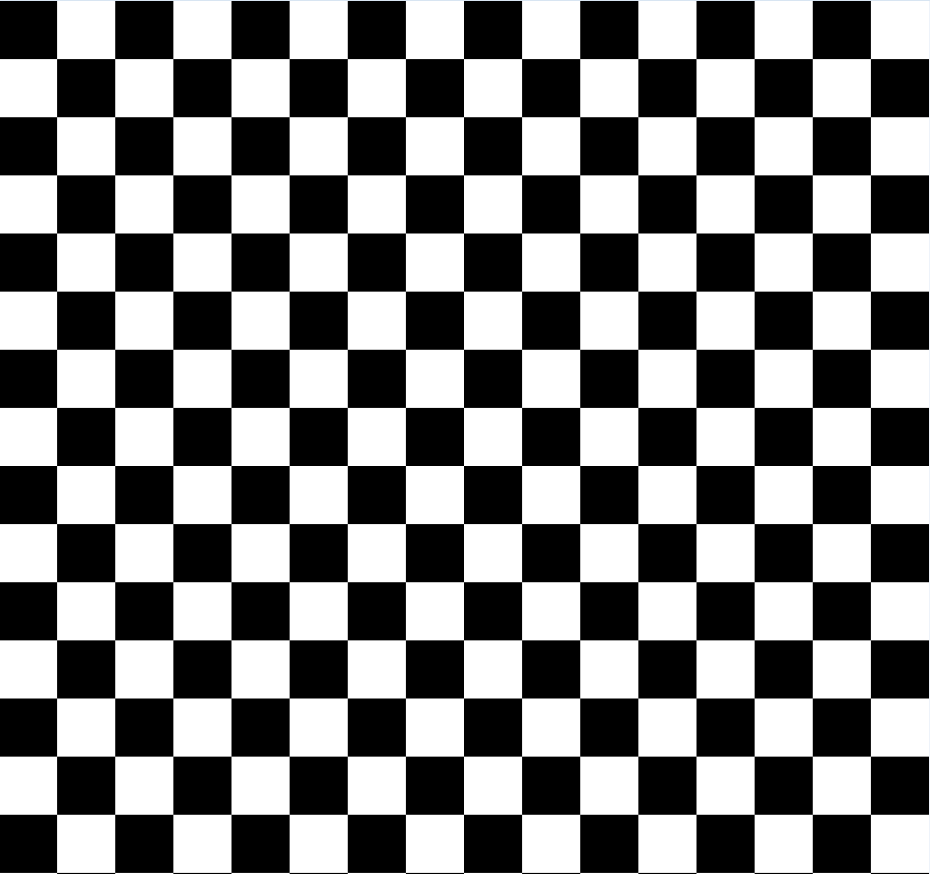
\includegraphics[width=0.30\textwidth]{checker1.png}
    \caption{An image of a checkerboard. Image taken from [\cite{dip}].}
    \label{checker1}
\par}
\end{figure}

% If we slice a strip on the image we can represent it as an one dimensional signal as shown in figure({\ref{checker2}) below.

% \begin{figure}[!htb]
%     {\centering
%         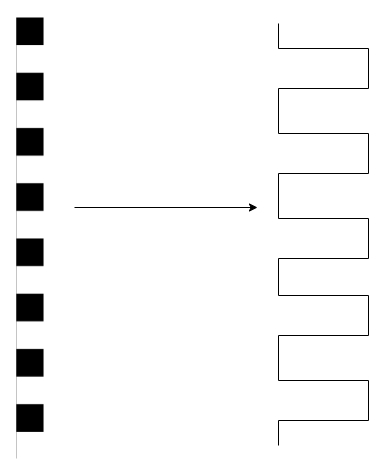
\includegraphics[width=0.30\textwidth]{checker2.png}
%         \caption{By taking a slice of the image we can represent it as an pulse.}
%         \label{checker2}
%     \par}
%     \end{figure}

If we sample with less pixels (or increase the frequency rate(the rate of changing intensities) of the object we are imaging) we could end up with only getting every cycle of the black intensity such that we only get a black strip. We could also use a different sampling rate and end up getting an $"$Fake$"$ image by reconstructing every second black intensity with one white in between such as shown in the sliced checkerboard in figure (\ref{checker3}) below.
\begin{figure}[!htb]
    {\centering
        
\includegraphics[width=0.30\textwidth]{checker3.png}
        \caption{Aliased slice}
        \label{checker3}
    \par}
    \end{figure}
By sampling with less pixels we could end up having the $"$same$"$ image, but with a longer period between the intensities. This also applies to resizing because when we resize down an image we need to remove pixels, which would destroy some of the information in the image. If we then resize it to the original shape we would apply interpolation and would most likely change the real intensity valued pixels to some other neighboring pixel value and therefore damage the quality of the image.

\subsection{2}

In figure 4.19 in the book [\cite{dip}] we can clearly see the aliasing effect in the area of the high frequency pixels. On the scarf, pants and the chair in the background the intensity values changes rapidly(high frequency). Therefore when resizing we would change the sampling rate below the Nyquist and lose information which we cant retrieve when resizing back to original shape.

\subsection{3}


We resize the image to 50\% of its original size, the result can be shown in figure(\ref{resized}) . The resizing is done by only taking out every second pixel in the original image into an new image.

\begin{figure}[!htb]
    {\centering
        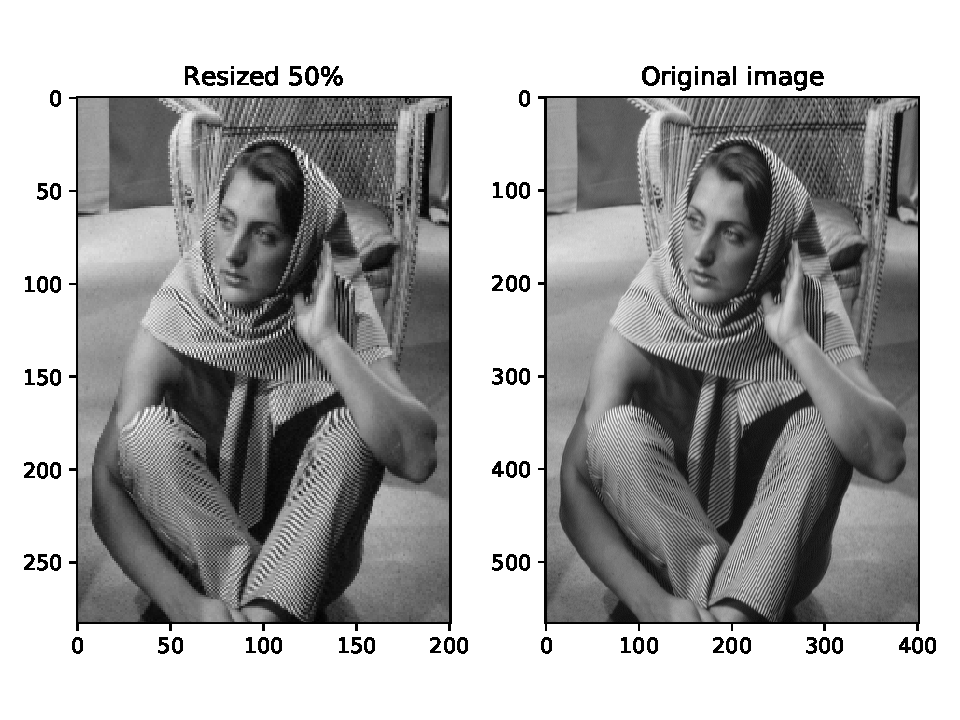
\includegraphics[width=0.60\textwidth]{resized.pdf}
        \caption{Resized image to 50\% of its original size, we can clearly observe the aliasing in the high frequency areas of the image.}
        \label{resized}
    \par}
    \end{figure}

In the figure we can see the aliasing effect as the high frequency areas wont be sampled at the right sampling rate to observe the rapid changing pattern.

\subsection{4}

We can blur the images prior to resizing by convolving an averaging filter with the image as follows,
\begin{figure}[!htb]
\begin{equation}
    g(x,y) = h(x,y) \bigstar i(x,y)
\end{equation}
\end{figure}

where h is the average filter defined as in equation(\ref{avaragefilter}) and i(x,y) is the image, $\bigstar$ means convolution. 

\begin{figure}[!htb]
\begin{equation}
    h = \frac{1}{MN}\begin{bmatrix}
        1_{1,1}       & 1_{1,2} & 1_{1,3} & \dots & 1_{N,1} \\
        1_{1,2}       & 1_{2,2} & 1_{3,2} & \dots & 1_{N,2} \\
        \hdotsfor{5} \\
        1_{1,M}       & 1_{2,M} & 1_{3,M} & \dots & 1_{N,M}
    \end{bmatrix}
    \label{avaragefilter}
\end{equation}
\end{figure}

when convolving we are applying the filter in the spatial domain, since this is an averaging filter/moving averaging(as it traverses the image), we essentially apply a lowpass filter. Lowpass filter will only allow the low frequency components of the image to go through. This means that the image will not have rapid changing intensities(more smudged out/smooth). This is clearly visible in figure(\ref{smooth}). This will decrease the effect of aliasing. In fact this is how many of the anti-aliasing setting in video games work.[\cite{wiki}]
When applying a filter we want to zero pad our image, in the case of convolving in spatial domain we would have problems fitting the kernel on the edges of the image. In our case the the convolve method from scipy module in python does this.

\begin{figure}[!htb]
    \begin{lstlisting}
        # Convolve using scipy package
        from scipy.signal import convolve2d
        mask = conconvolve2d(image, Laplacian, mode = 'same')
    \end{lstlisting}
\end{figure}

\begin{figure}[!htb]
    {\centering
        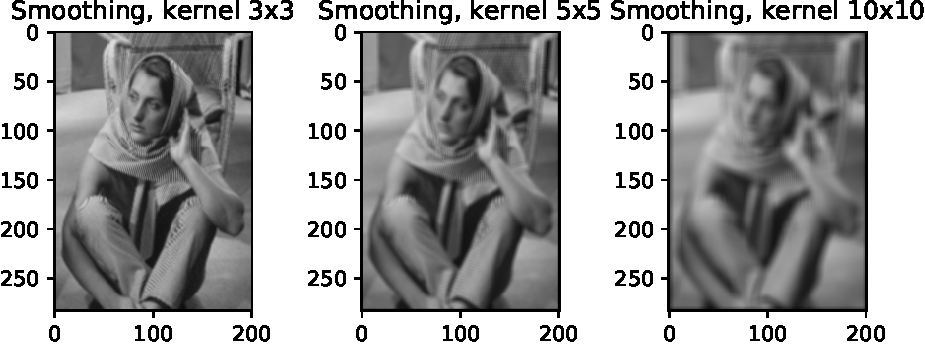
\includegraphics[width=0.95\textwidth]{smoothing.pdf}
        \caption{Smoothed the aliased image with different sizes of the averaging kernel. We can see here that the 10x10 kernel has strong blurring. The aliasing seems to go away as we blur the image.}
        \label{smooth}
    \par}
    \end{figure}

\subsection{5}

We can try to restore the image by using an sharpening filter we would emphasize the edges better by using filters such as Laplace. Laplace is a second order derivative so here we would emphasize pixels with high frequency and de-emphasize areas with low frequency (high pass filter). We use the Laplace kernel given in equation(\ref{laplace kernel}),

\begin{equation}
    h = \begin{bmatrix}
        1 & 1 & 1 & \\
        1 & -8 & 1\\
        1 & 1 & 1
    \end{bmatrix}
    \label{laplace kernel}
\end{equation}

This stems from the fact that we use the Laplacian $\nabla^2 f(x,y)$ which will generate the discrete version $f[x,y+1] + f[x+1,y+1] + f[x+1,y] + f[x-1,y] + f[x-1,y-1] + f[x+1,y-1] - 4f[x,y]$(summing to zero yield no response in areas of constant intensity). This is linear and therefore allowed to be used in convolution. By doing this convolution we get a mask g(x,y),

\begin{figure}[!htb]
    \begin{equation}
        g(x,y) = h(x,y) \bigstar i(x,y)
    \end{equation}
    \end{figure}

here h(x,y) is the Laplacian filter and i(x,y) is the image. To enhance the edges we add this mask to our image. By using the Laplace kernel in equation(\ref{laplace kernel}) we will sharpen in all direction. We could for instance use a star-shaped Laplace to neglect diagonal direction. (set diagonals in the matrix to zero.)

\begin{figure}[!htb]
    \begin{equation}
        E(x,y) = i(x,y) + Cg(x,y)
    \end{equation}
    \end{figure}
Where E(x,y) is the enhanced image and C is an constant which is either -1 or 1 depending on which Laplacian kernel we use. In this case $c = -1$.

The result of the sharping with two different methods are shown in figure(\ref{sharpened}).

\begin{figure}[!htb]
    {\centering
        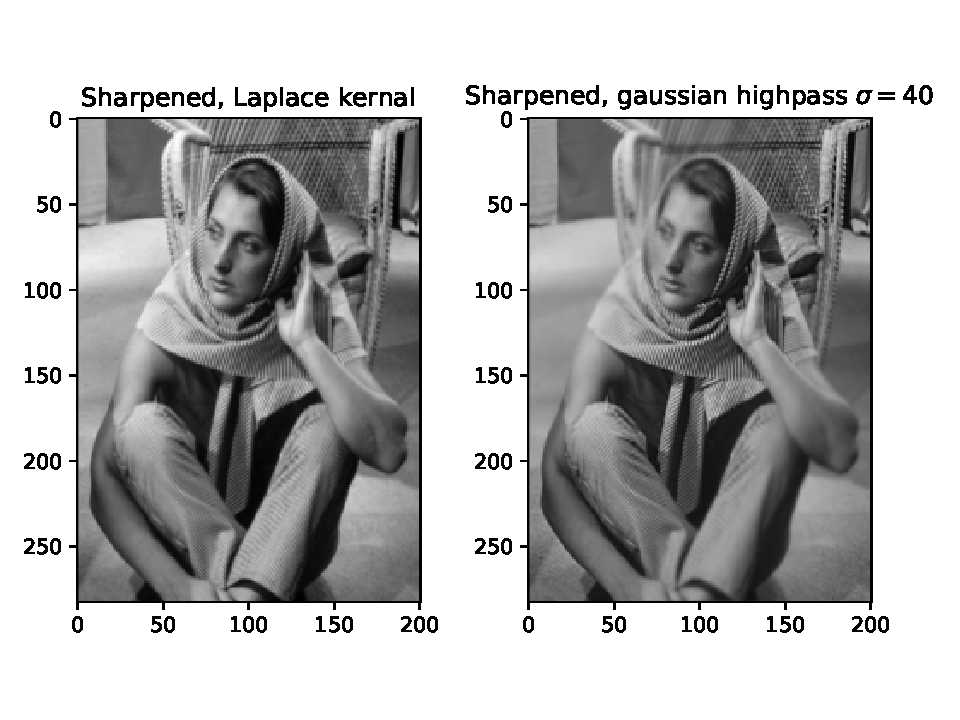
\includegraphics[width=0.80\textwidth]{sharpened.pdf}
        \caption{Sharpened by using two different sharping techniques. Remark: Laplace sharping was done in spatial domain and gaussian high pass was done in frequency domain.}
        \label{sharpened}
    \par}
    \end{figure}

In this figure we can see that it has more defined edges. The gaussian high pass sharpening method contains more blurring, but we could tune the parameter $\sigma$(cut off) to fit better. The image is much better then the resized version which contained aliasing.

The gaussian high pass filter uses the gaussian function (which is a lowpass filter),

\begin{equation}
    H_{lp}(u,v) = e^{D^2/2\sigma^2}
    \label{gausslowp}
\end{equation}
This function is in the frequency domain, D is the distance from the centered frequency and $\sigma$ is the radius parameter. To get the high pass filter we need to subtract it from one.

\begin{equation}
    H_{hp}(u,v) = (1 - H_{lp})
    \label{gausshighp}
\end{equation}

To apply this filter we multiply it by the centered frequency domain representation of the image I(u,v).

\begin{equation}
    G(x,y) =  (1 - H_{lp})I(u,v)
\end{equation}

This will yield a mask which contains the high frequencies. We then sum this on our original image to sharpen the edges.

In the previous case we blurred the image PRIOR to resizing, this made the image look good and without aliasing. We have these images in figure(\ref{smooth2}).

\begin{figure}[!htb]
    {\centering
        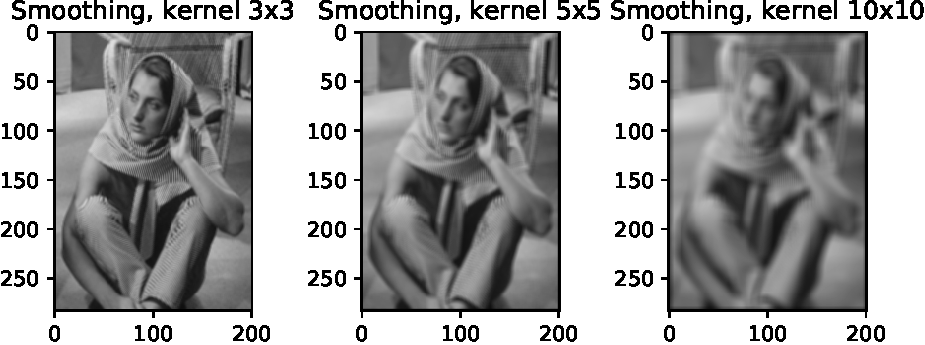
\includegraphics[width=0.90\textwidth]{smoothafter.pdf}
        \caption{Smoothed images on images blurred after resizing.}
        \label{smooth2}
    \par}
    \end{figure}

If we blur the image after resizing and using Laplace sharping we get the images in figure(\ref{sharpened2}).

\begin{figure}[!htb]
    {\centering
        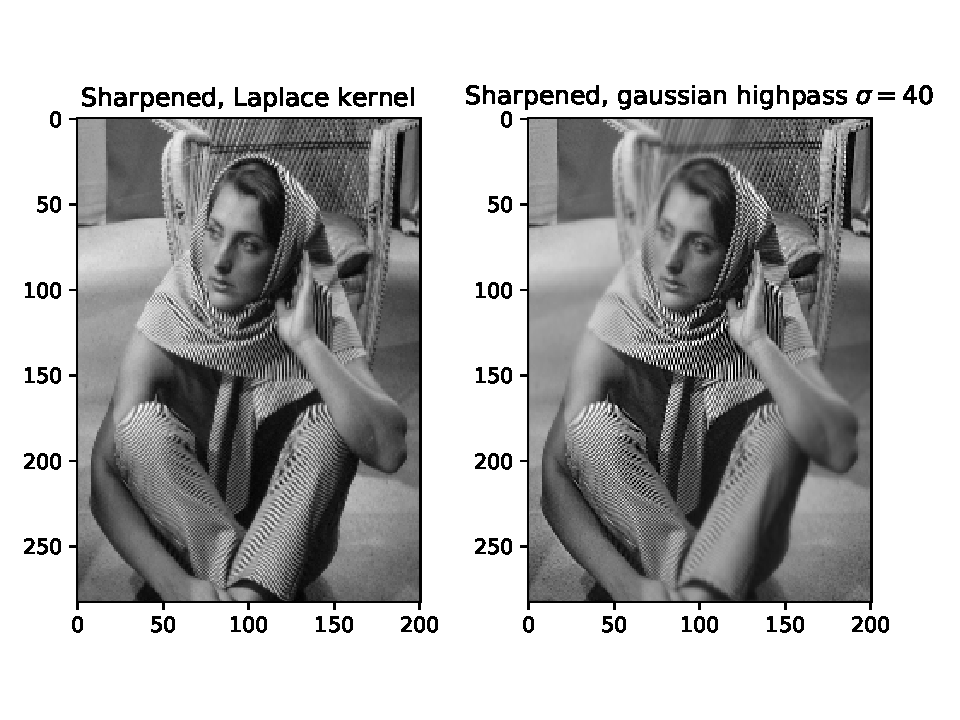
\includegraphics[width=0.60\textwidth]{sharpened2.pdf}
        \caption{Sharpened by using two different sharping techniques on image blurred after resizing. Here we can clearly see that we got aliasing again.}
        \label{sharpened2}
    \par}
    \end{figure}
In this case we can see that the aliasing is back, so here we can see how sharpening works counter to blurring.


\section{Part C}
\subsection{1}


By visually inspecting the images,in \emph{F1.png} we can clearly see the distinctive \emph{salt \& pepper} noise with its black/white broken pixels. In \emph{F2.png} it looks like gaussian noise, in \emph{F3.png} we have vertical periodic noise, in \emph{F4.png} we have horizontal periodic noise. In the last image \emph{F5.png} we have a superposition of horizontal and vertical periodic noises. The images of shown in figure(\ref{Fimages}).


\begin{figure}[!htb]
    {\centering
    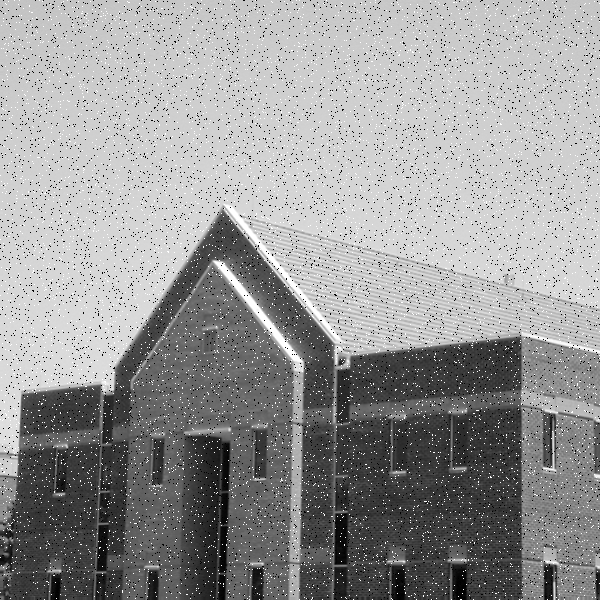
\includegraphics[width=0.30\textwidth]{F1.png} \,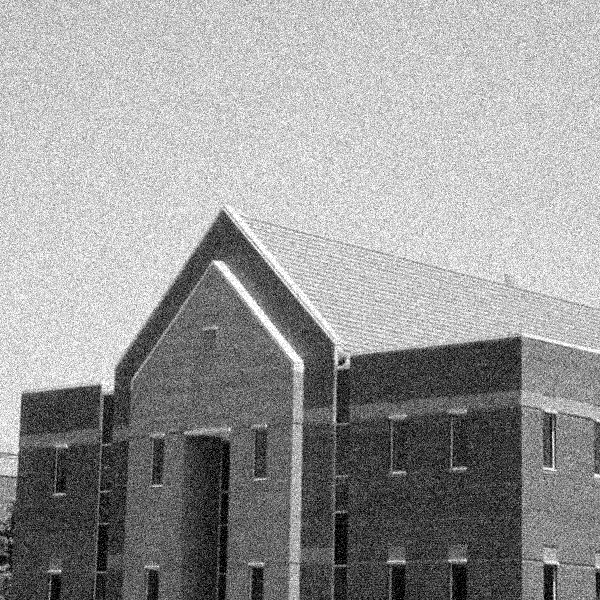
\includegraphics[width=0.30\textwidth]{F2.png}\\ 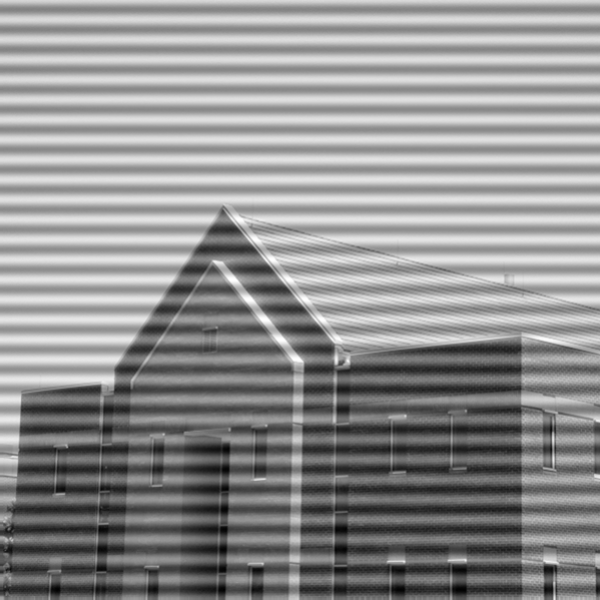
\includegraphics[width=0.30\textwidth]{F3.png} \,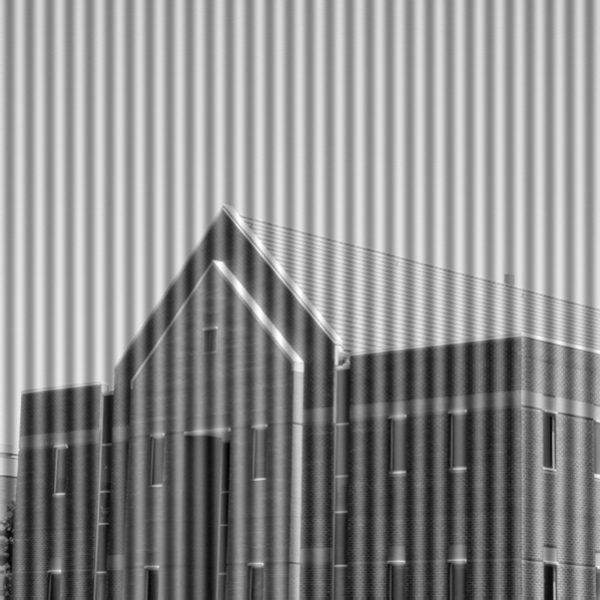
\includegraphics[width=0.30\textwidth]{F4.png}\\ 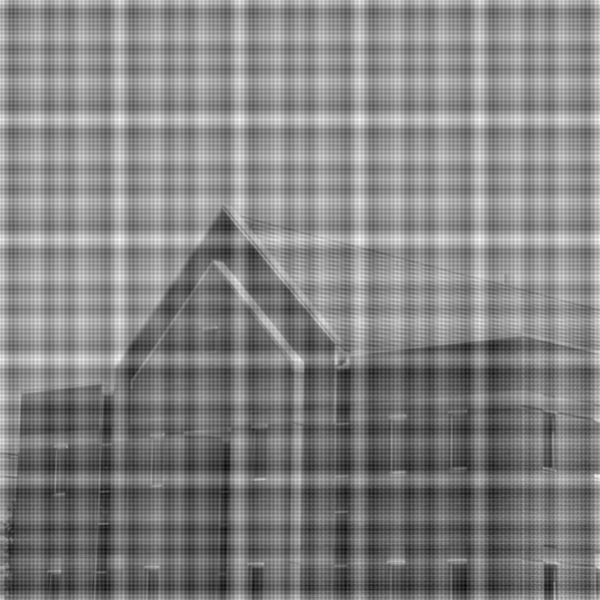
\includegraphics[width=0.30\textwidth]{F5.png}
        \caption{Image F1.png, F2.png, F3.png, F4.png, F5.png}
        \label{Fimages}
    \par}
    \end{figure}



We could find the histogram representation of the image to see the noise pattern, in figure(\ref{histogramnoise}) we can see that the gaussian noise form gaussian structures in the histogram. The salt and pepper noise has large spike at the white and black intensity(0 and 255), but the overall structure of the image stays intact, its much harder to know the structure of the image with the gaussian noise.
\begin{figure}[!htb]
    {\centering
        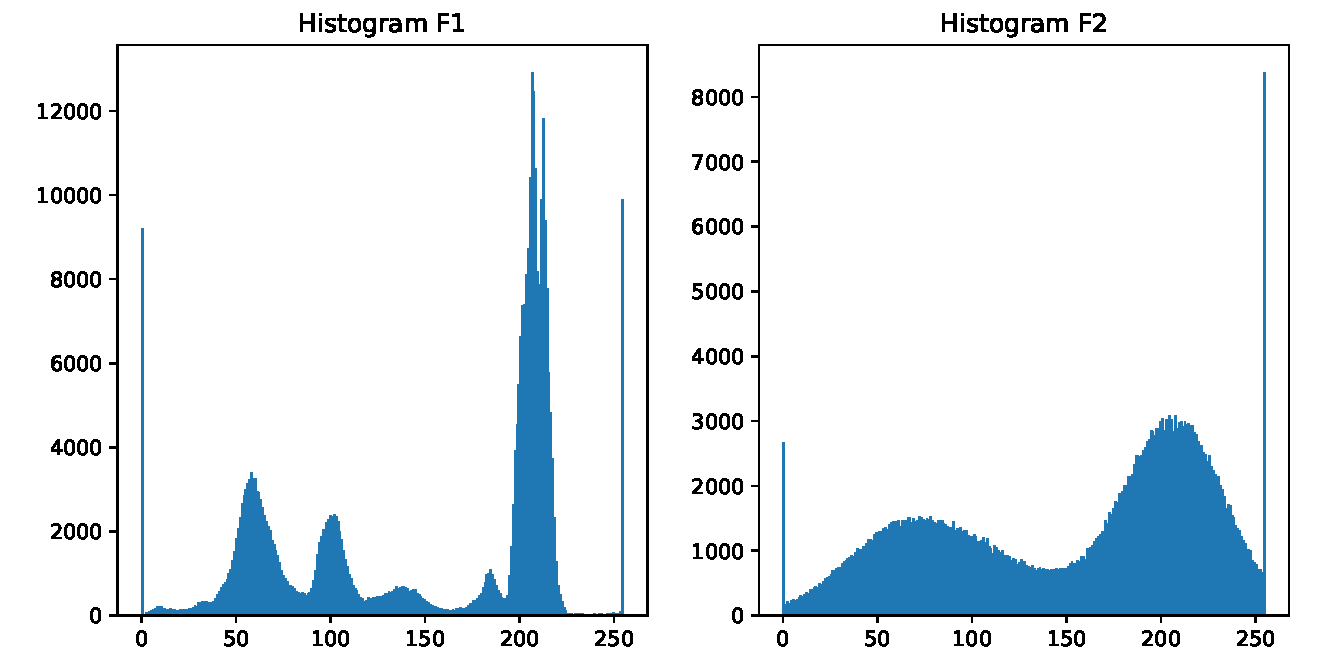
\includegraphics[width=0.70\textwidth]{noisehist.pdf}
        \caption{Histogram of the images}
        \label{histogramnoise}
    \par}
    \end{figure}

The periodic noises would be a lot easier to see in the frequency domain as sine waves in frequency domain look like conjugated impulses. In figure(\ref{fourierrep}) we can see the impulses.

    \begin{figure}[!htb]
        {\centering
            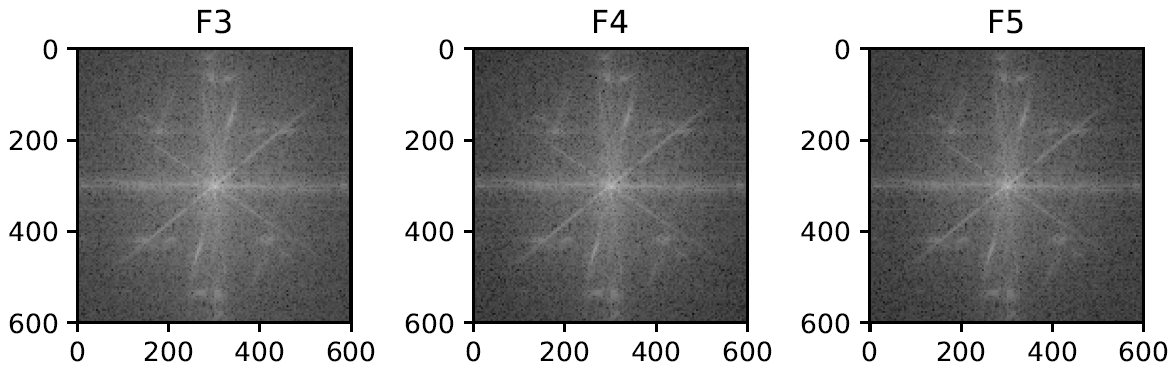
\includegraphics[width=0.95\textwidth]{fourierrep.png}
            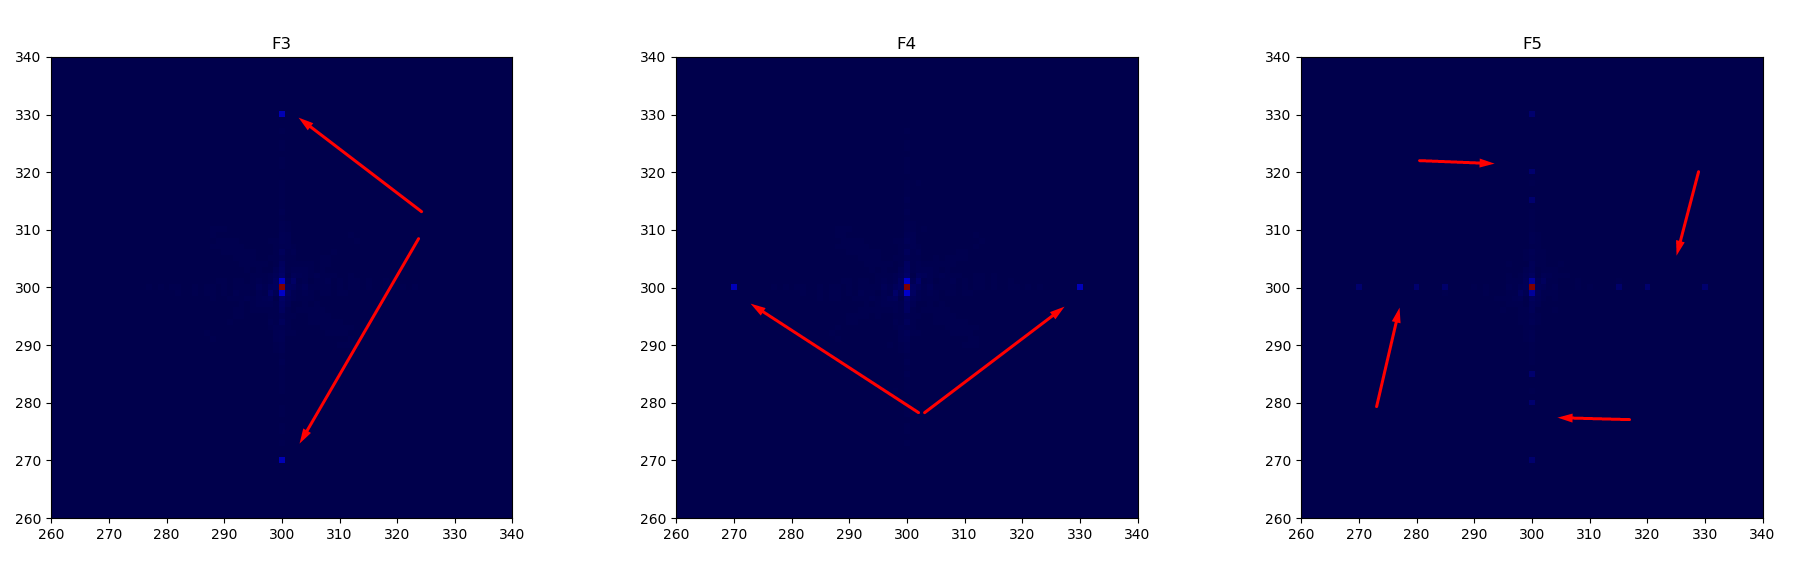
\includegraphics[width=0.95\textwidth]{filterrep2.png}
            \caption{First row show the frequency representation of the images in dB scale. If we do not use dB scale we get higher difference between the energy of the spectrum, but by zooming in we can clearly see the impulses from the periodic noise.}
            \label{fourierrep}
        \par}
        \end{figure}


\subsection{2}

For removing salt and pepper noise a median filter would be a good choice. With the median filter we rank the values from lowest to highest value and choose the 50\% percentile intensity value in the kernel and set this value as the new pixel intensity of the new image. We do this for all the pixels in the image.


\begin{figure}[!htb]
    {\centering
        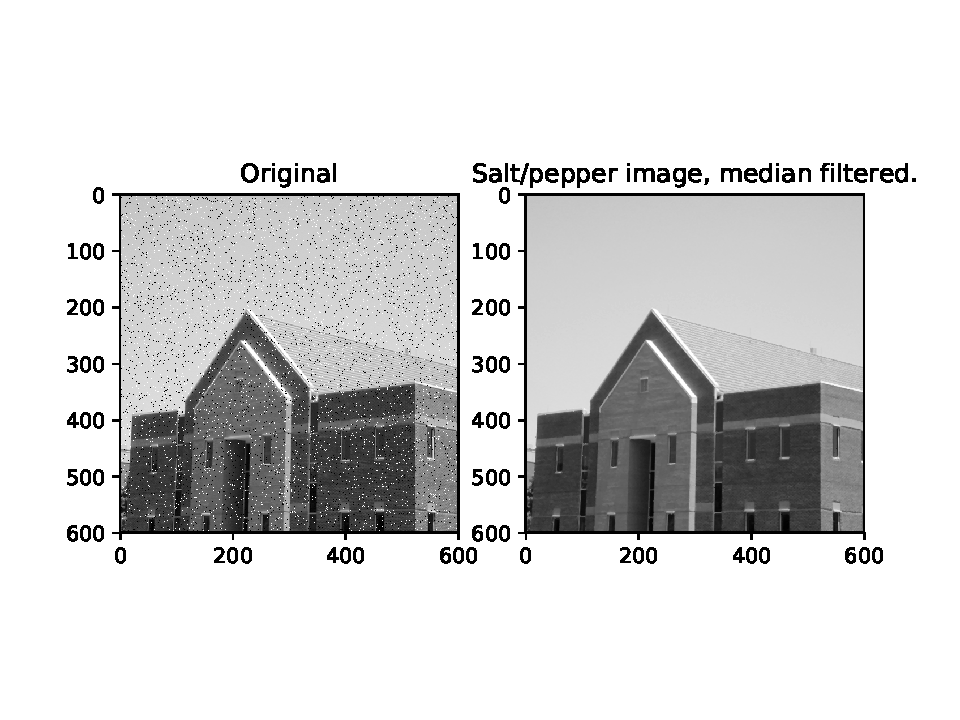
\includegraphics[width=0.72\textwidth]{Filtered_saltimage.pdf}
        \caption{F1 image filtered using median filter with a 3x3 kernel.}
        \label{salt}
    \par}
    \end{figure}
Here g(r,c) is the values from the image which are inside our convolving kernel.

For the gaussian noise image we use an adaptive filter defined as,

\begin{equation}
    \hat{f}(x,y) = g(x,y) - \frac{\sigma^{2}_{\eta}}{\sigma_{S_{xy}}}\left[g(x,y) - \bar{z}_{S_{xy}}\right]
    \label{adaptive}
\end{equation}

Here $\hat{f}(x,y)$ is the filtered image, $g(x,y)$ is the noisy image, $\sigma^{2}_{\eta}$ is the variance of the noise, $\sigma_{S_{xy}}$ is the variance inside the kernel which is traversing the image, $\bar{z}_{S_{xy}}$ is the mean in of the kernel. Here we found the estimated variance of the noise by finding the variance in an sub image which taken to be the top part of the image which has mostly low frequency in the original image. The variance was found with the sample variance in equation(\ref{variance}).

\begin{equation}
    \hat{\sigma}^{2}_{\eta} = \sum_{i = 0}^{N-1}\frac{(r_{i} - \bar{r})^{2}}{N-1}
    \label{variance}
\end{equation}
where r is the intensity value and $\bar{r}$ is the mean intensity value.


\begin{figure}[!htb]
    {\centering
        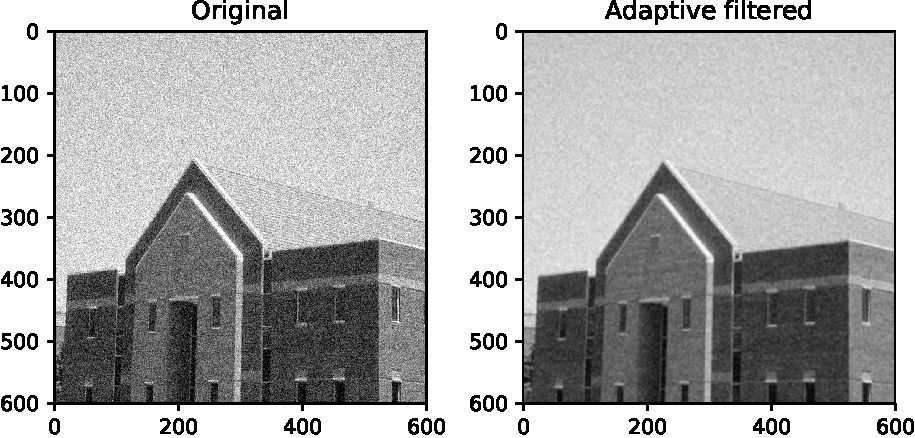
\includegraphics[width=0.72\textwidth]{gaussianfiltered.pdf}
        \caption{Filtered gaussian noise image, here we applied the adaptive filter discussed above. }
        \label{adaptivefig}
    \par}
    \end{figure}

It looks better, but we could probably do better with some other technique. If we look at the histogram in figure(\ref{histogramnoise}) we might suspect that we have salt \& pepper + gaussian noise.


\subsection{3}

The procedure for filtering in frequency domain is,

\begin{itemize}
    \item 1. Obtain the image f(x,y) which is of size MxN.
    \item 2. Calculate new dimensions P and Q, P = 2M, Q = 2N.
    \item 3. Pad image i(x,y) to dimensions PxQ with zeros-, mirror-, or replicate padding. mirror padding will mirror the pixels at the borders. Pad the image at the bottom and right side to make it easier to slice out the image later.
    \item 4. Shift the image to center it in frequency domain, this makes it easier to do the multiplication right. This is done by multiplying the image as such $i(x,y)(-1)^{x+y}$.
    \item  5. Compute the DFT to obtain I(u,v).
    \item 6. Obtain a symmetric filter function in the frequency domain, H(u,v) of dimension PxQ. This should also be centered at P/2 Q/2! If the filter is made in spatial domain do the same procedure as the image.
    \item 7. Filtering in spatial domain is done by convolving, which is the same as multiplying in the frequency domain. Filter the image by forming the product G(x,y) = I(u,v)H(u,v)(elementwise product).
    \item 8. To obtain the filtered image in spatial domain we do the \emph{inverse} discrete Fourier transform (IDFT), we now have g(x,y).
    \item shift the image back to original position by $g(x,y)(-1)^{x+y}$ and take the real part/absolute value.
    \item 9. Slice out the image by taking out the top left part of the image with size MxN. We now have the filtered image $\hat{i}(x,y)$.
\end{itemize}

When zero padding it does not matter how we apply them around the image, what matters is how many zeros. When using the discrete Fourier transforms we run into an periodicity problem. This will in effect make our signal/image repeat every $1/(2\Delta t)$ in frequency domain (we use 1D for simplicity) where $\Delta t$ is the sampling rate in time. As mentioned earlier convolution in time is multiplication in frequency domain. When convolving we shift our filter back and flip it 180$\degree$. In equation(\ref{contconv}) we have the continues definition of the convolution.

\begin{equation}
    x(t) \bigstar h(t) = \int_{-\infty}^{\infty} x(\tau)h(t - \tau)\, d\tau
    \label{contconv}
\end{equation}
or the DFT in equation(\ref{discconv}),

\begin{equation}
    x[n] \bigstar h[n] = \sum_{m = 0}^{M-1} x(m)h(n - m)
    \label{discconv}
\end{equation}

but since we work with the discrete version we now have this sequence in periodic intervals, this means that when we perform the convolution we do a convolution with its periodicities. Although we can multiply them in the frequency domain we have to perform the inverse to get the image, which will in turn do the circular convolution which will yield a wrap around error. If we zero pad the signal/image in spatial/time domain we increase the distance to its periodicity such that the convolution is finished before it arrives at the periodicity generated from the DFT.


\subsection{4}

Since both salt \& pepper noise and gaussian noise has high frequency using a gaussian low pass (see equation(\ref{gausslowp}))would help removing a lot of the noise as shown in figure(\ref{task4gauss}) and figure(\ref{task4pepper}).

\begin{figure}[!htb]
    {\centering
        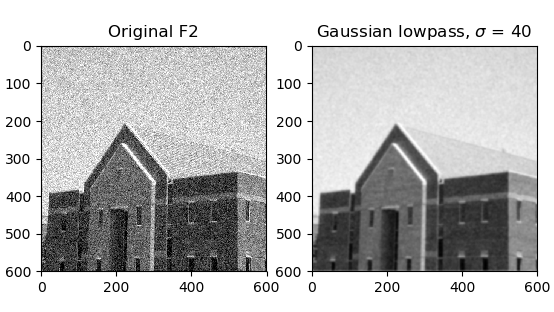
\includegraphics[width=0.75\textwidth]{task4gauss.png}
        \caption{Original image to the left and frequency representation on the left. We can observe the two conjugated impulse representing the periodic component in the image.}
        \label{task4gauss}
    \par}
    \end{figure}



    \begin{figure}[!htb]
        {\centering
            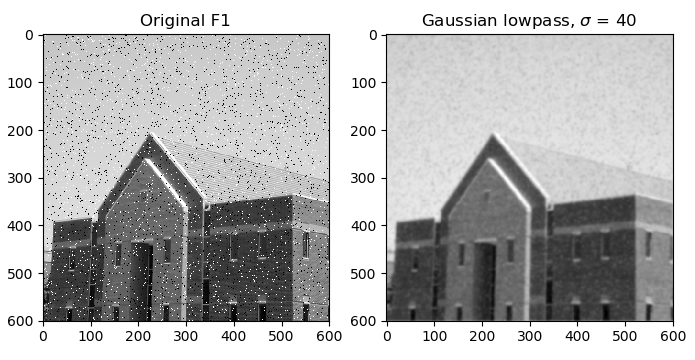
\includegraphics[width=0.75\textwidth]{task4pepper.png}
            \caption{Original image to the left and frequency representation on the left. We can observe the two conjugated impulse representing the periodic component in the image.}
            \label{task4pepper}
        \par}
        \end{figure}

Although we removed much noise we now have very smooth borders on the building, we could use a Butterworth filter instead of the gaussian to try and tweak with the right parameters to get sharper edges. The salt and pepper noise were easier to remove in spatial domain with the median filter as it kept the image sharp and clean.

\subsection{5}


The noise in F3 and F4 are the same noise except one is shifted by $90\degree$, by analyzing F4 in the frequency domain, see figure(\ref{fourierrep}) we can see that there are some conjugated impulses. These impulses are shifted to $\approx$ +- 20 from the center, so here we have a period of about 20 pixels between the amplitudes of the noise. If we inspect the spatial domain we can also see that the lines are separated by $\approx$ 20 pixels between the amplitudes so in F3 and F4 we have a frequency of 0.05.

\begin{figure}[!htb]
    {\centering
        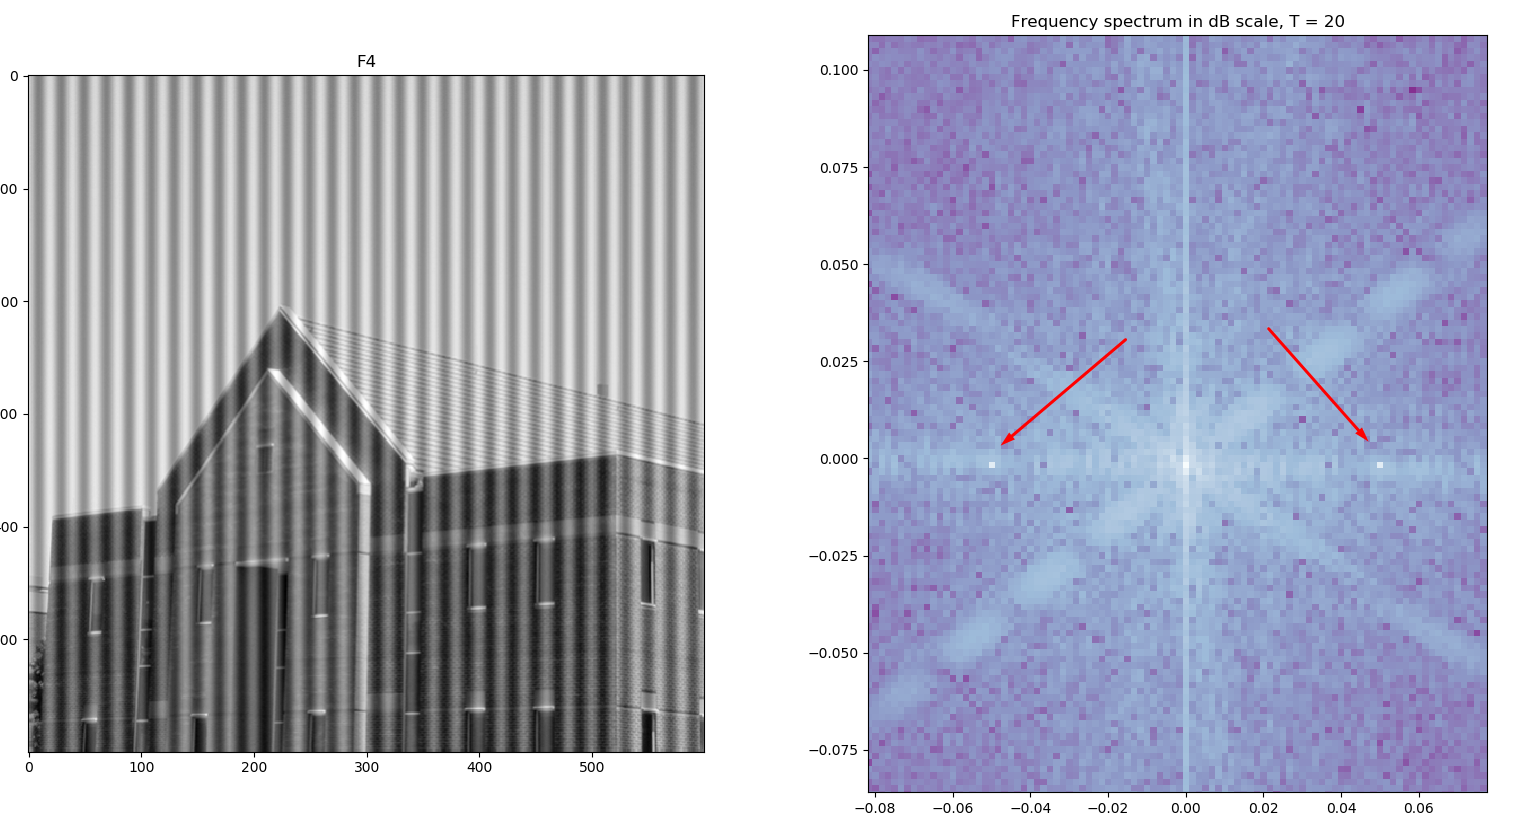
\includegraphics[width=0.75\textwidth]{simulatedperiod.png}
        \caption{Original image to the left and frequency representation on the left. We can observe the two conjugated impulse representing the periodic component in the image. The impulses are at -0.05 and 0.05.}
        \label{simulatedperiod}
    \par}
    \end{figure}




\subsection{6}


We can clearly see in the frequency domain of the image F5 the impulses of the periodic noise of the image in figure(\ref{F5period}). It looks like we have 8 periodic components 4 horizontal and 4 vertical.


\begin{figure}[!htb]
    {\centering
        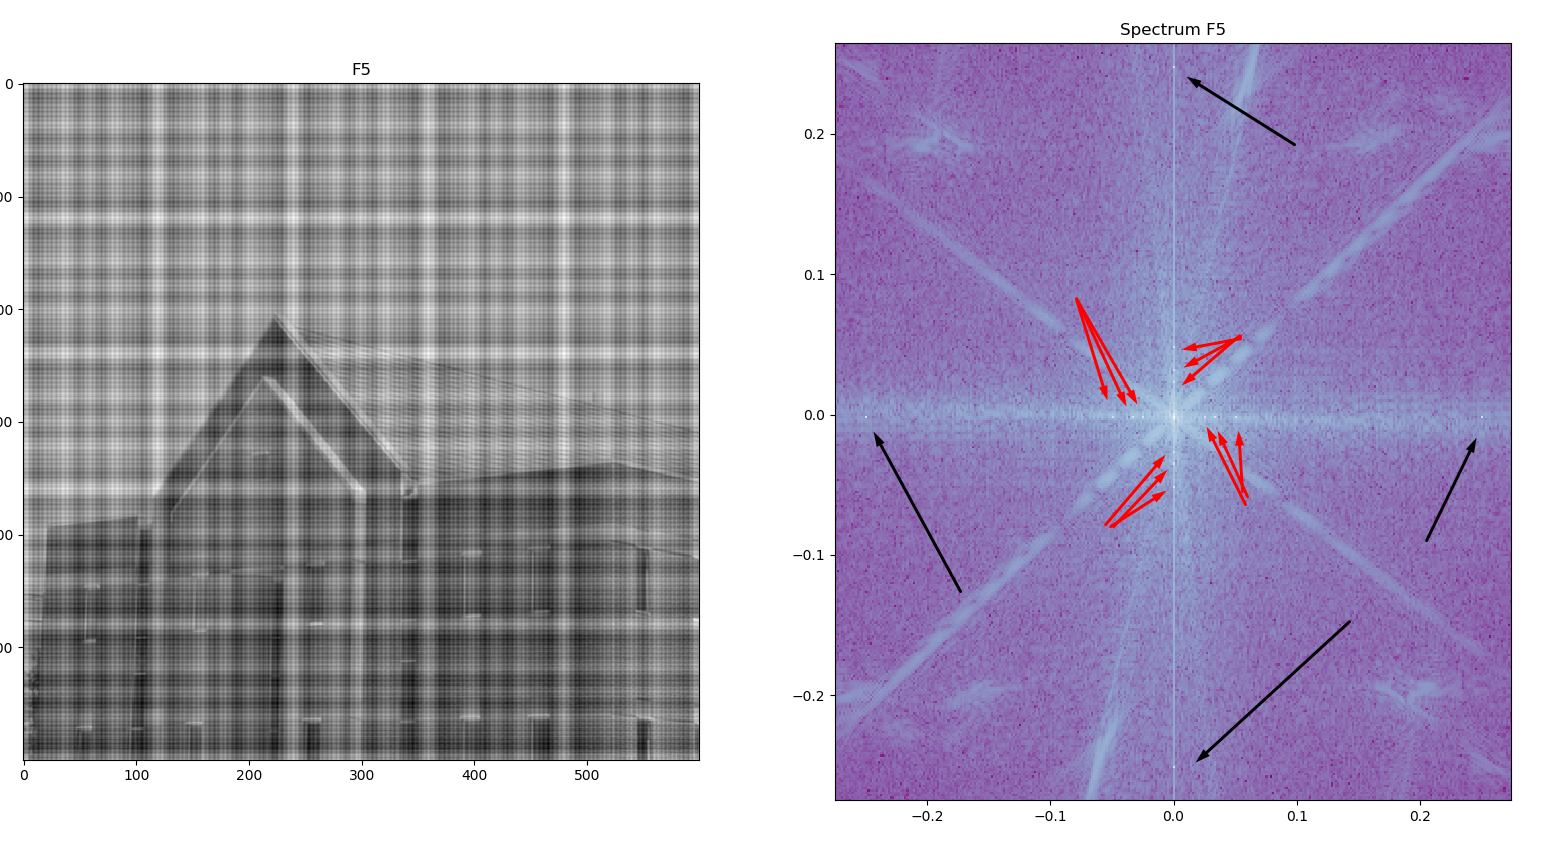
\includegraphics[width=0.75\textwidth]{superpositionfreq.png}
        \caption{Left; Original image F5, Right; decibel frequency domain. The black arrows show 2 periodicities with high frequency}
        \label{F5period}
    \par}
    \end{figure}


The frequencies are, $\approx \textit{vertical}\{0.25, 0.05, 0.03, 0.02\}, \textit{horisontal}\{0.25, 0.05, 0.03, 0.2\}$.





\subsection{7}

%F3

For filtering the images in this task we used the Butterworth notch reject filter,

\begin{equation}
    H_{NR}(u,v) = \prod_{k=1}^{3}\left[\frac{1}{1+[D_{0k}/D_{k}(u,v)]^{n}} \right]\left[\frac{1}{1+[D_{0k}/D_{-k}(u,v)]^{n}} \right]
    \label{notchiboy}
\end{equation}

where $D_{0k}$ is the cutoff frequency for each notch, $D_{k}(u,v) $is the distance to the impulse to place the notch, these are symmetric so we have a $D_{-k}(u,v)$ term as well, and n is the order of Butterworth.

Removing the noise in all the images below was done with this filter (with cutoff 1 and order $n = 3$), on each of the impulses. Shown in figure(\ref{C7F3freq}) we have the frequency domain representation of the image F3. The result of using this notch filter on F3 is shown in figure(\ref{C7F3}).

\begin{figure}[!htb]
    {\centering
        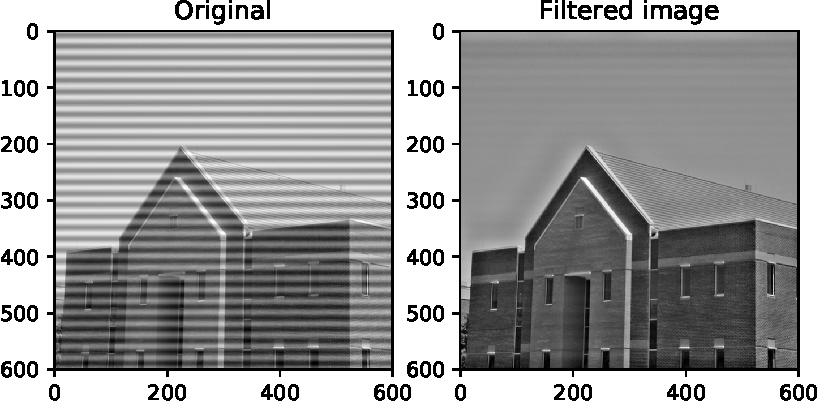
\includegraphics[width=0.80\textwidth]{C7F3.pdf}
        \caption{Left; Original image, Right; Filtered image, here we managed to remove almost all the noise. For removing the noise we used equation(\ref{notchiboy}) with $D_{0} = 1$ and $n = 3$.  We have also sharpened using equation(\ref{sharping2}) with $k = 1$ and in our high pass Butterworth $n = 5$, $D_{0} = 8$.}
        \label{C7F3}
    \par}
    \end{figure}



    \begin{figure}[!htb]
        {\centering
            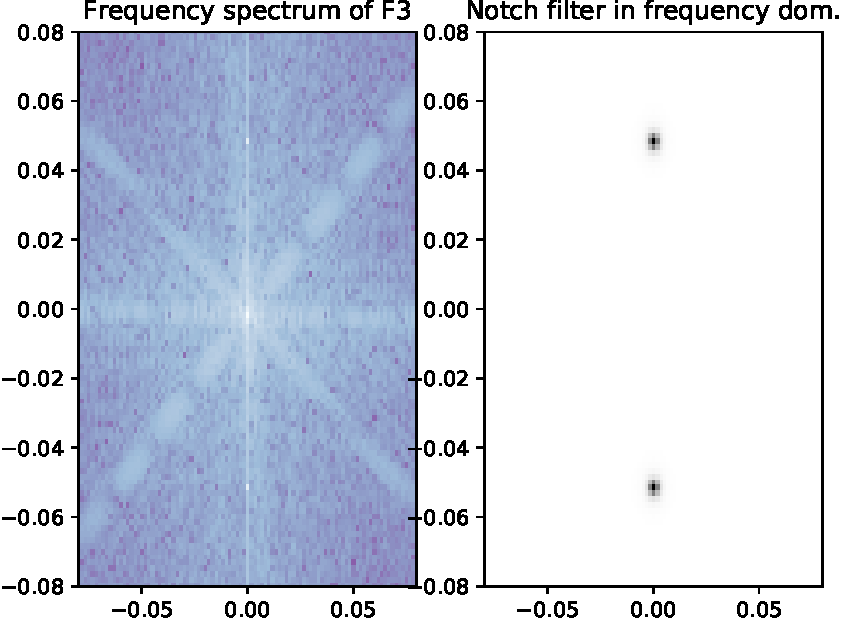
\includegraphics[width=0.55\textwidth]{C7F3freq.pdf}
            \caption{Left; frequency representation of image F5.png, Right; frequency representation of the Butterworth notch filter. Here we have vertical impulses since the periodic noise is in y-direction.}
            \label{C7F3freq}
        \par}
        \end{figure}

    After applying notch rejection and sharpening we transformed the intensities to 0-255 using equation(\ref{transform}).
\begin{equation}
    g(x,y) = \frac{image-min\{image\}}{max\{image-min\{image\}\}}(L-1)
    \label{transform}
\end{equation}

where $L = 256$ in this case.

The sharpening is done by the high-frequency-emphasis filtering in equation(\ref{sharping2}),

\begin{equation}
    g(x,y) = \mathcal{F}^{-1}\left\lbrace[1 + kH_{HP}(u,v)]F(u,v) \right\lbrace
    \label{sharping2}
\end{equation}

Here $\mathcal{F}^{-1}$ is the inverse Fourier transform, k gives control over the proportion of high frequencies. When we applied this we used $k = 1$ and g(x,y) is the sharpened image, and F(u,v) is the frequency domain of the noise filtered image.


As the high pass filter we used the Butterworth high pass filter given by equation(\ref{buttyboi} ,

\begin{equation}
   H_{HP} = \frac{1}{1+[D_{0}/D(u,v))]^{2n}}
    \label{buttyboi}
\end{equation}

Here $D(u,v)$ is the distance from the center, $D_{0}$ is the cutoff frequency and n is the order of the filter, the higher this order is the closer to ideal filter. The closer to ideal filter we are the more ringing effect will we have.

%F4

Image F4.png is almost the same noise, but shifted by $90\degree$, so here we flip our previous notch filter and apply and then sharpen with equation(\ref{sharping2}), the result is shown in figure(\ref{C7F4}).

\begin{figure}[!htb]
    {\centering
        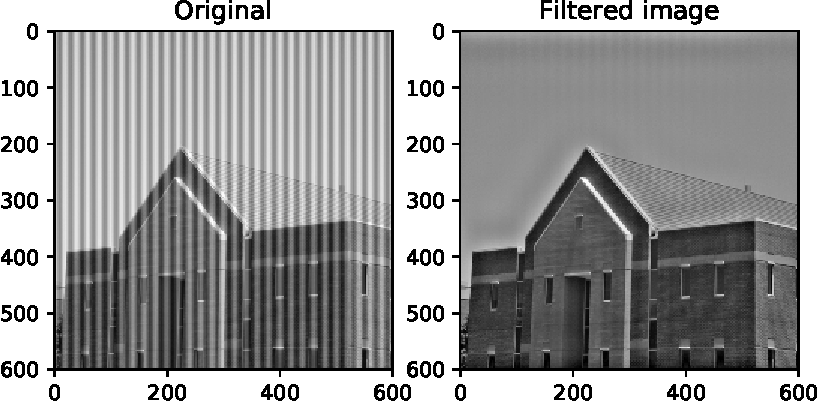
\includegraphics[width=0.85\textwidth]{C7F4.pdf}
        \caption{Left; Original image, Right; Filtered image, here we managed to remove almost all the noise. For removing the noise we used equation(\ref{notchiboy}) with $D_{0} = 1$ and $n = 3$. We have also sharpened using equation(\ref{sharping2}) with $k = 1$ and in our high pass Butterworth $n = 5$,$D_{0} = 8$.}
        \label{C7F4}
    \par}
    \end{figure}

    \begin{figure}[!htb]
        {\centering
            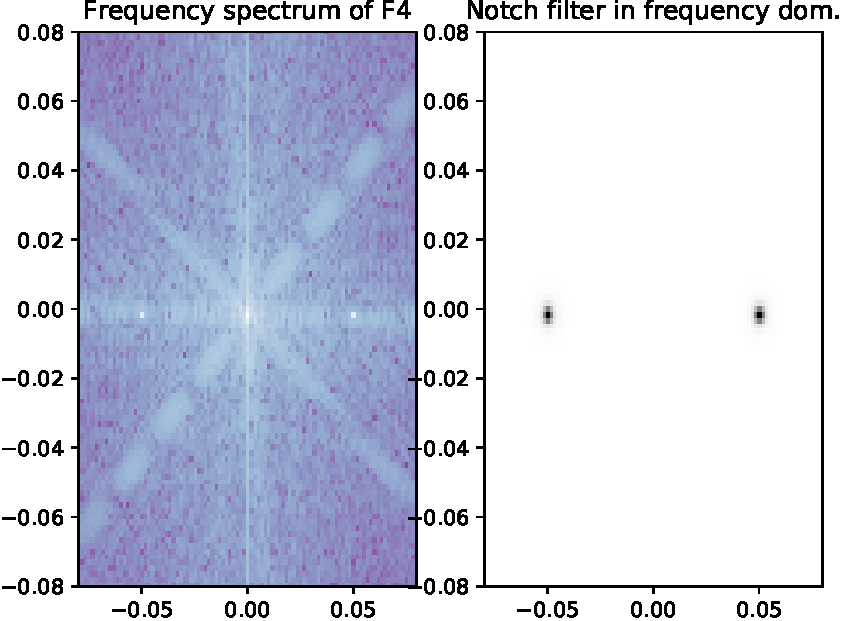
\includegraphics[width=0.65\textwidth]{C7F4freq.pdf}
            \caption{Left; frequency representation of image F4.png, Right; frequency representation of the Butterworth notch filter. Here the impulses are in horizontal direction since the noise is periodic in x-direction.}
            \label{C7F4freq}
        \par}
        \end{figure}


Removing the noise in image F5 was done by using a Butterworth notch filter (with cutoff 1 and order $n = 3$), on each of the 8 impulses shown in figure(\ref{F5notch}). As we can see in figure(\ref{C7F5}) we have removed almost all the noise, we have some ripple effects in some areas, most likely because we used notches which were to idealized, so here we should have tried other parameters to tune it better.


\begin{figure}[!htb]
    {\centering
        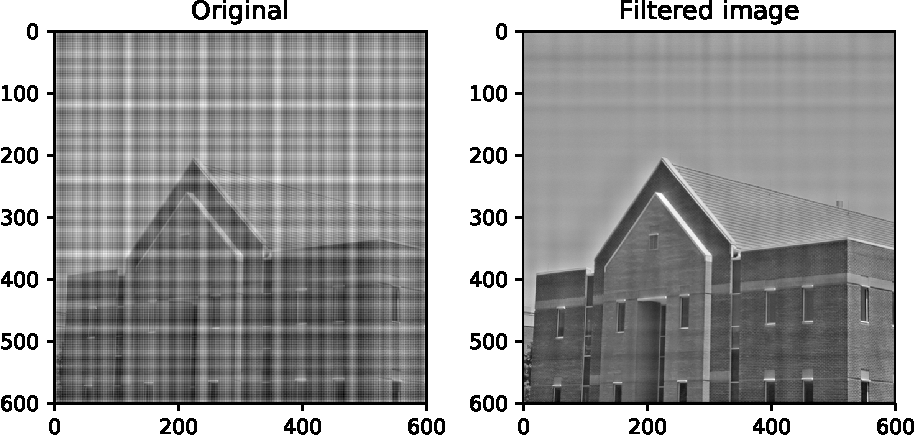
\includegraphics[width=0.80\textwidth]{C7F5.pdf}
        \caption{Left; Original image, Right; Filtered image, here we managed to remove almost all the noise. For removing the noise we used equation(\ref{notchiboy}) with $D_{0} = 1$ and $n = 3$. We have also sharpened using equation(\ref{sharping2}) with $k = 1$ and in our high pass Butterworth $n = 5$, $D_{0} = 8$.}
        \label{C7F5}
    \par}
    \end{figure}

After removing the noise with the notch filter, we made a edge mask using Butterworth with cutoff 7 and order $n = 5$.



In figure(\ref{F5notch}) we see the dB scale frequency spectrum and the Butterworth notch rejection filter applied. Her we can see the black dots applied right on top of the impulses generated from the periodic noise.

    \begin{figure}[!htb]
        {\centering
            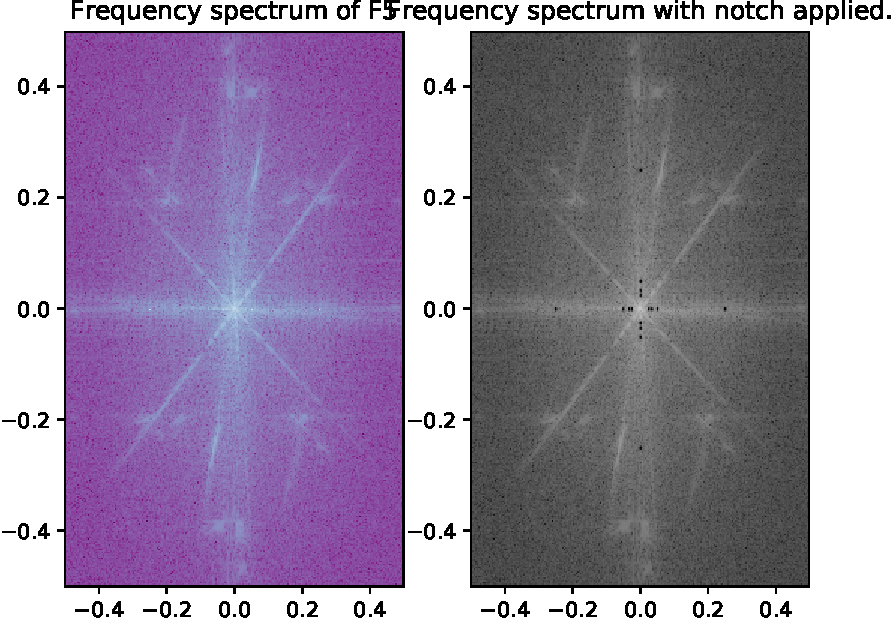
\includegraphics[width=0.65\textwidth]{removed_per_noise_freq.pdf}
            \caption{Left; frequency representation of image F5.png, Right; frequency representation with the Butterworth notch reject filter applied.}
            \label{F5notch}
        \par}
        \end{figure}






\section{Part D}
\subsection{1}







% --------------------------------------------------------------
%     Reference og appendix
% --------------------------------------------------------------
\newpage
\section{Appendix}



\section{Part A}









\section{References}
\begingroup
\renewcommand{\section}[2]{}%
%\renewcommand{\chapter}[2]{}% for other classes
\bibliographystyle{plainnat}
\bibliography{bibl}
\endgroup















% --------------------------------------------------------------
%     You don't have to mess with anything below this line.
% --------------------------------------------------------------
 





\end{document}


